\section{Mosaic Design}
TODO: Phases...

\subsection{Phase I}
TODO

\subsection{Phase II}
TODO

\subsection{Phase III}
TODO

\subsection{Liquidity Simulation Environment}
TODO

\subsubsection{Liquidity Forecasting}
We recently launched Mosaic’s Proof of Concept (PoC) and are currently collecting valuable data to help improve user experience as cross-chain and cross-layer token swaps are made. To help decide on a usable fee model, we have also introduced our Liquidity Simulation Environment (LSE), a software toolkit capable of running simulated swaps.

Through the recent work of Composable Labs, we have advanced the LSE and built in a forecasting mechanism which can predict in advance when a certain liquidity level will be reached for a given layer. This will be critical for the optimization of the passive liquidity rebalancing that will enable passive liquidity providers to continue to service cross-layer transfers.

Having an optimal allocation of capital across layers is, thus, key to offering the best performance for users seeking to move cross-layer. Therefore, understanding when said capital reaches certain key levels where action will need to be taken is important.

By leveraging data collected from the LSE, we have learned how we can improve our vault mesh grid, Mosaic, for the users benefits. This will allow us to maximize the number of successful token transfers for users, providing a seamless user experience when transferring assets.

To start using data from our LSE, we employed an autoregressive integrated moving average (ARIMA) model to fit and forecast liquidity data on the Polygon vault. Our time series data consisted of 1000 liquidity observations obtained on an hourly basis.

This data observation collection is similar to the approach we took when discovering our alpha strategy utilizing SushiSwap LP (SLP) tokens — but now simulated instead. To recap our simulated approach, we select a number of token movements in the vaults of our LSE. These movements are drawn from a truncated Gaussian with parameters set to resemble those real-world transfers.

As an aside, the Mosaic PoC is intended to provide even more realistic data and can be mixed in with simulations or used on its own; we leave that for future work.

After gathering the simulated data, we snapped the information to a global time grid. Then we used a state machine to evolve the vaults forward in time starting at pre-defined initial/seed liquidity levels. This gave rise to evolving liquidity levels over time which can be seen in Fig.~(\ref{fig:forecast1}).
%
\begin{figure}
    \centering
    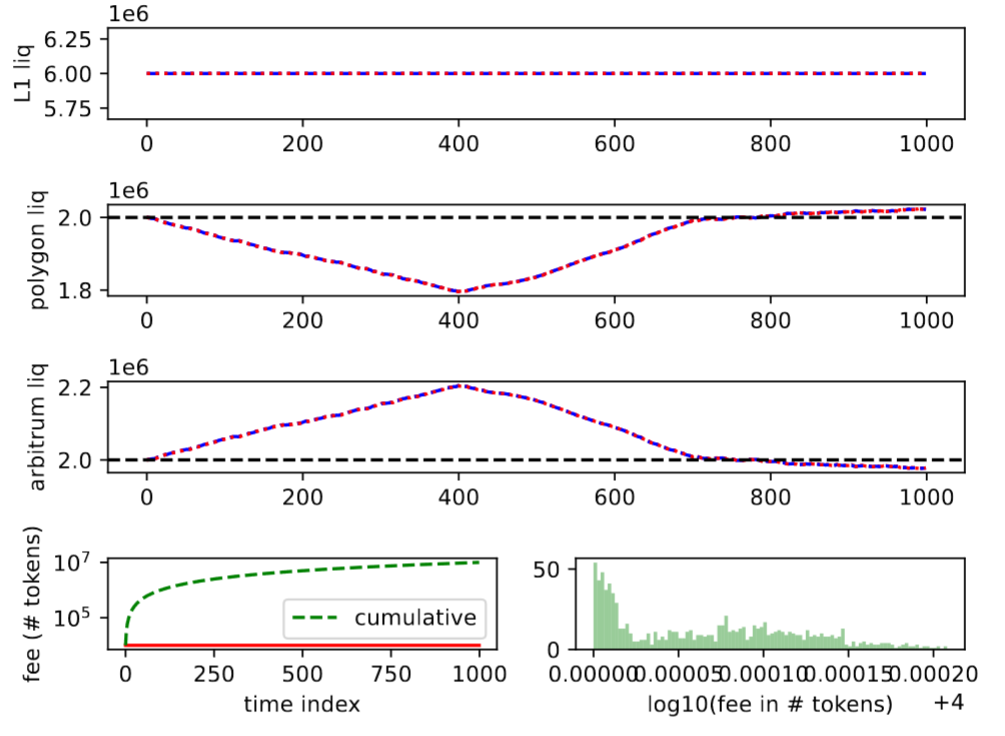
\includegraphics[width=15cm]{images/mosaic/forecast1.png}
    \caption{Caption}
    \label{fig:forecast1}
\end{figure}
%
For this forecasting exercise, we used 200 training points (roughly eight days worth of data) each time we fit an ARIMA model, and we use it to forecast on a time horizon of 168 hours (roughly one week ahead) which coincides with some layer 2 (L2) to layer 1 (L1) exit times.

After repeated trial and error attempts, and using the Akaike information criterion (AIC) for comparison between the models, we found that an ARIMA (20, 1, 20) model would work well.

From here, the model was then fit on our data using maximum likelihood. For the forecasting, we used a standard normal distribution for sampling on the inferred model parameters and then propagated our prediction from the current time to 168 hours in the future.

Using our equation, we were able to create a forecasting model for the need of liquidity on Polygon. In the model shown below, the red confidence interval is one week worth of forecasting from having trained on eight days of data. The blue full line is data collected to aid in this forecast.
%
\begin{figure}
    \centering
    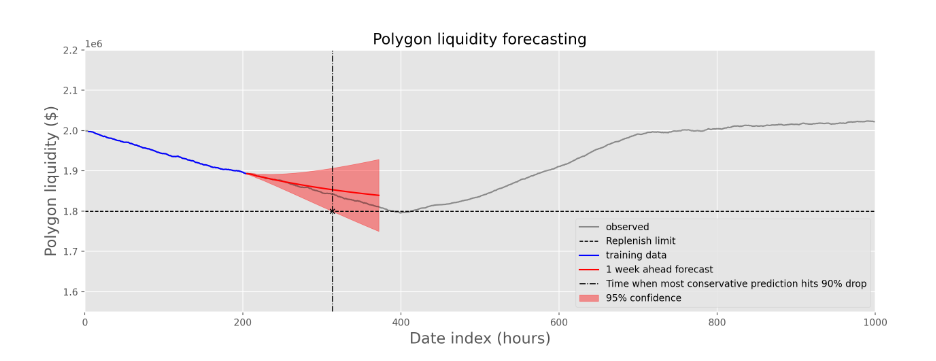
\includegraphics[width=15cm]{images/mosaic/forecast2.png}
    \caption{Caption}
    \label{fig:forecast1}
\end{figure}
%
For this model, we chose 200 data points as the training data (shown in blue) and fit these points in our ARIMA model. The red triangular-esque region is the forecasted values with the red full line being the mean liquidity prediction and the shaded red area the confidence intervals.

The black point shows where the model predicts that a 90\% liquidity level is reached in the vault by conservative estimates (the lower confidence level). We keep the model conservative which explains the wide confidence level.

This prediction can be used to trigger a replenishment event in advance. The idea is to trigger said event (replenish the L2 vault from L1) when the liquidity level hits the 90\% level, or \$1.8 million in this case.
%
\begin{figure}
    \centering
    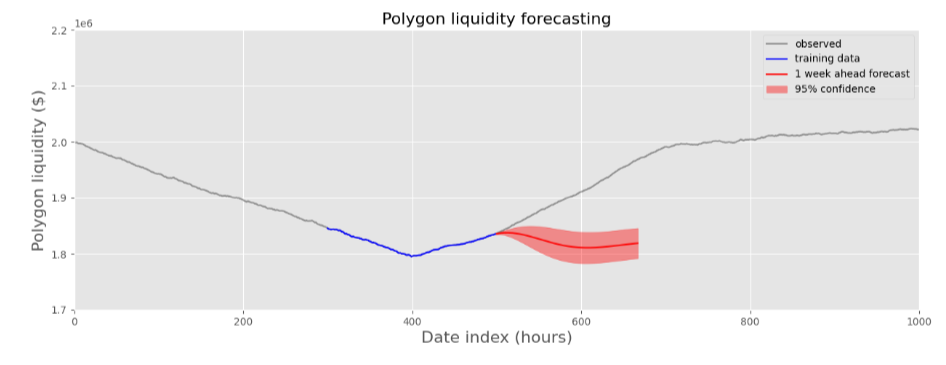
\includegraphics[width=15cm]{images/mosaic/forecast3.png}
    \caption{Caption}
    \label{fig:forecast1}
\end{figure}
%

\subsubsection{Fee Model}
TODO
